\section{Estado de la cuestión}\label{cap:estado_cuestion}

En la actualidad existen diversas soluciones tecnológicas relacionadas con la Semana Santa, aunque la mayoría de ellas se encuentran limitadas a ámbitos geográficos concretos o se centran únicamente en la difusión de información estática. A continuación, se analizan las principales herramientas disponibles, así como sus características más relevantes.

\subsection{Aplicaciones actuales de Semana Santa}

A día de hoy, existen diversas aplicaciones móviles orientadas a la Semana Santa para distintas ciudades españolas. Entre ellas encontramos \textit{El Penitente} \cite{elpenitente}, centrada únicamente en las ciudades de Sevilla y Málaga. Esta aplicación ofrece información sobre horarios, itinerarios y una representación del recorrido de las procesiones sobre el mapa, mostrando el trayecto seguido y, en algunos casos, su posición aproximada.

La aplicación presenta una interfaz (Figura \ref{fig:penitente}) en la que el usuario puede consultar información sobre las procesiones y sus recorridos, avisos y notificaciones, planificaciones para organizar la Semana Santa y horarios de hermandades o cofradías.

\begin{figure}[ht!]
\centering
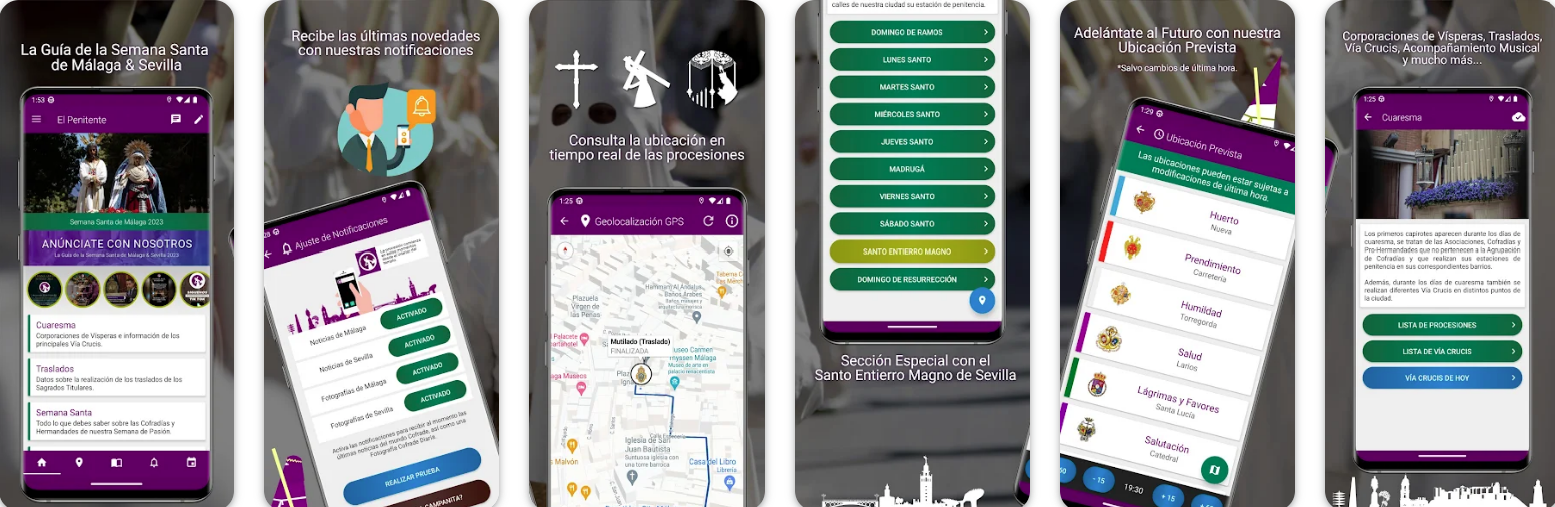
\includegraphics[width=0.9\textwidth]{imagenes/el_penitente.png}
\caption{Interfaz de la aplicación El Penitente \cite{fotosElpenitente}}
\label{fig:penitente}
\end{figure}

Su mayor limitación es que está diseñada y pensada para ciudades específicas y no constituye una solución unificada a nivel nacional.

Otra aplicación a analizar es \textit{Valladolid Cofrade} \cite{valladolidCofrade}, una herramienta reciente desarrollada como aplicación web progresiva (PWA) \cite{queEsPWA}, es decir, una aplicación accesible desde el navegador que puede instalarse en el dispositivo y funcionar de forma similar a una aplicación nativa. Esta permite a los usuarios acceder a información sobre la Semana Santa sin realizar la instalación tradicional desde tiendas oficiales. La aplicación ofrece información sobre programas, recorridos y un sistema de avisos y notificaciones en tiempo real ante cambios o incidencias (Figura \ref{fig:valladolid_cofrade}).

\begin{figure}[ht!]
\centering
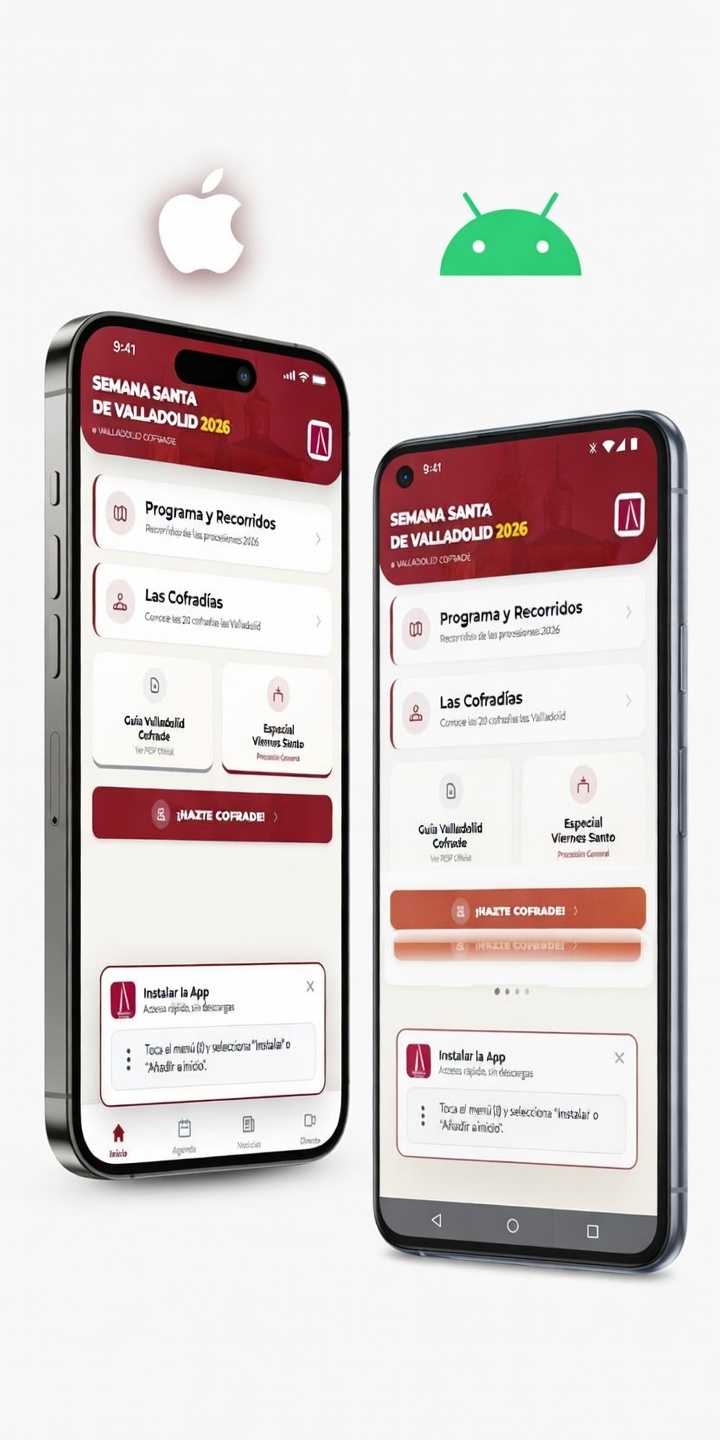
\includegraphics[width=0.4\textwidth]{imagenes/valladolid_cofrade.jpg}
\caption{Interfaz de la aplicación Valladolid Cofrade \cite{valladolidCofrade}}
\label{fig:valladolid_cofrade}
\end{figure}

En otras ciudades se cuenta con aplicaciones locales específicas o sitios web adaptados, como sSantaZgz en Zaragoza \cite{sSantaZgz} o Junta Pro Semana Santa de Zamora \cite{juntaZamora}. Estas aplicaciones muestran el programa oficial, los distintos recorridos e incluso, en algunos casos, como en la de Zamora, incluyen herramientas para conocer la previsión meteorológica.

Más allá de estas limitaciones técnicas, también hay que destacar la diversidad organizativa de la Semana Santa en España, ya que esta depende de la ciudad, de la estructura que se siga en ella y de la terminología utilizada. Por ejemplo, en algunas ciudades, como Valladolid, es común emplear los términos \textit{cofradía} o \textit{cofrade}, mientras que en otras, como Sevilla, se utilizan \textit{hermandad} o \textit{nazareno} para referirse a conceptos equivalentes. Desde el punto de vista organizativo, existen diferentes formas de organizar los eventos, recorridos e itinerarios de las procesiones. Incluso hay diferencias en elementos como pasos, imágenes, homilías, rezos o cánticos que forman parte de estas procesiones o eventos.

Estas diferencias hacen que cada aplicación tenga un diseño distinto, pensado específicamente para una ciudad concreta, dificultando la creación de una solución reutilizable. Por tanto, en la actualidad no existe una plataforma que consiga unificar y generalizar estos conceptos y ofrecer una visión global de la Semana Santa.

Además de las aplicaciones, los usuarios también hacen uso de las publicaciones oficiales de las cofradías en sus páginas web o de programas impresos. Sin embargo, los medios que realmente resultan útiles para la actualización inmediata de la información son las redes sociales oficiales de las cofradías o de las Juntas de Cofradías, que permiten a los espectadores recibir información sobre cambios o comunicados al instante. Aun así, esta forma de comunicación no siempre resulta fácil de encontrar o de organizar debido a la diversidad de cuentas que gestionan dicha información.

\subsection{Aplicaciones de seguimiento en tiempo real}

En cuanto a la geolocalización y el seguimiento en tiempo real, se trata de una tecnología ya existente que se utiliza en diversas aplicaciones como \textit{Google Maps} \cite{googlemapsapi}, que permite conocer la ubicación, cómo llegar a distintos destinos o el estado del transporte público (Figura \ref{fig:googlemaps}).

\begin{figure}[ht!]
\centering
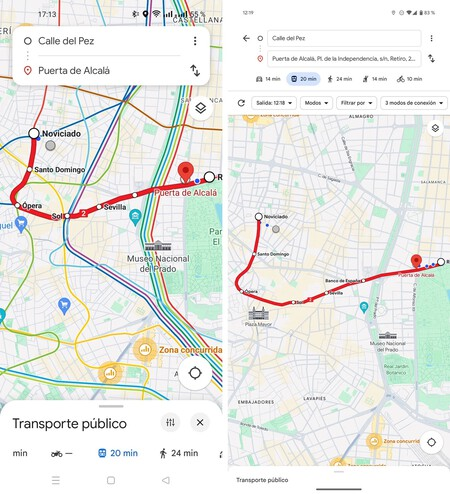
\includegraphics[width=0.6\textwidth]{imagenes/googlemaps.jpeg}
\caption{Ejemplo de geolocalización en tiempo real en Google Maps}
\label{fig:googlemaps}
\end{figure}

Además, plataformas como \textit{Uber} \cite{uber} permiten a los usuarios conocer en todo momento la ubicación exacta del vehículo solicitado (Figura \ref{fig:uber}).

\begin{figure}[ht!]
\centering
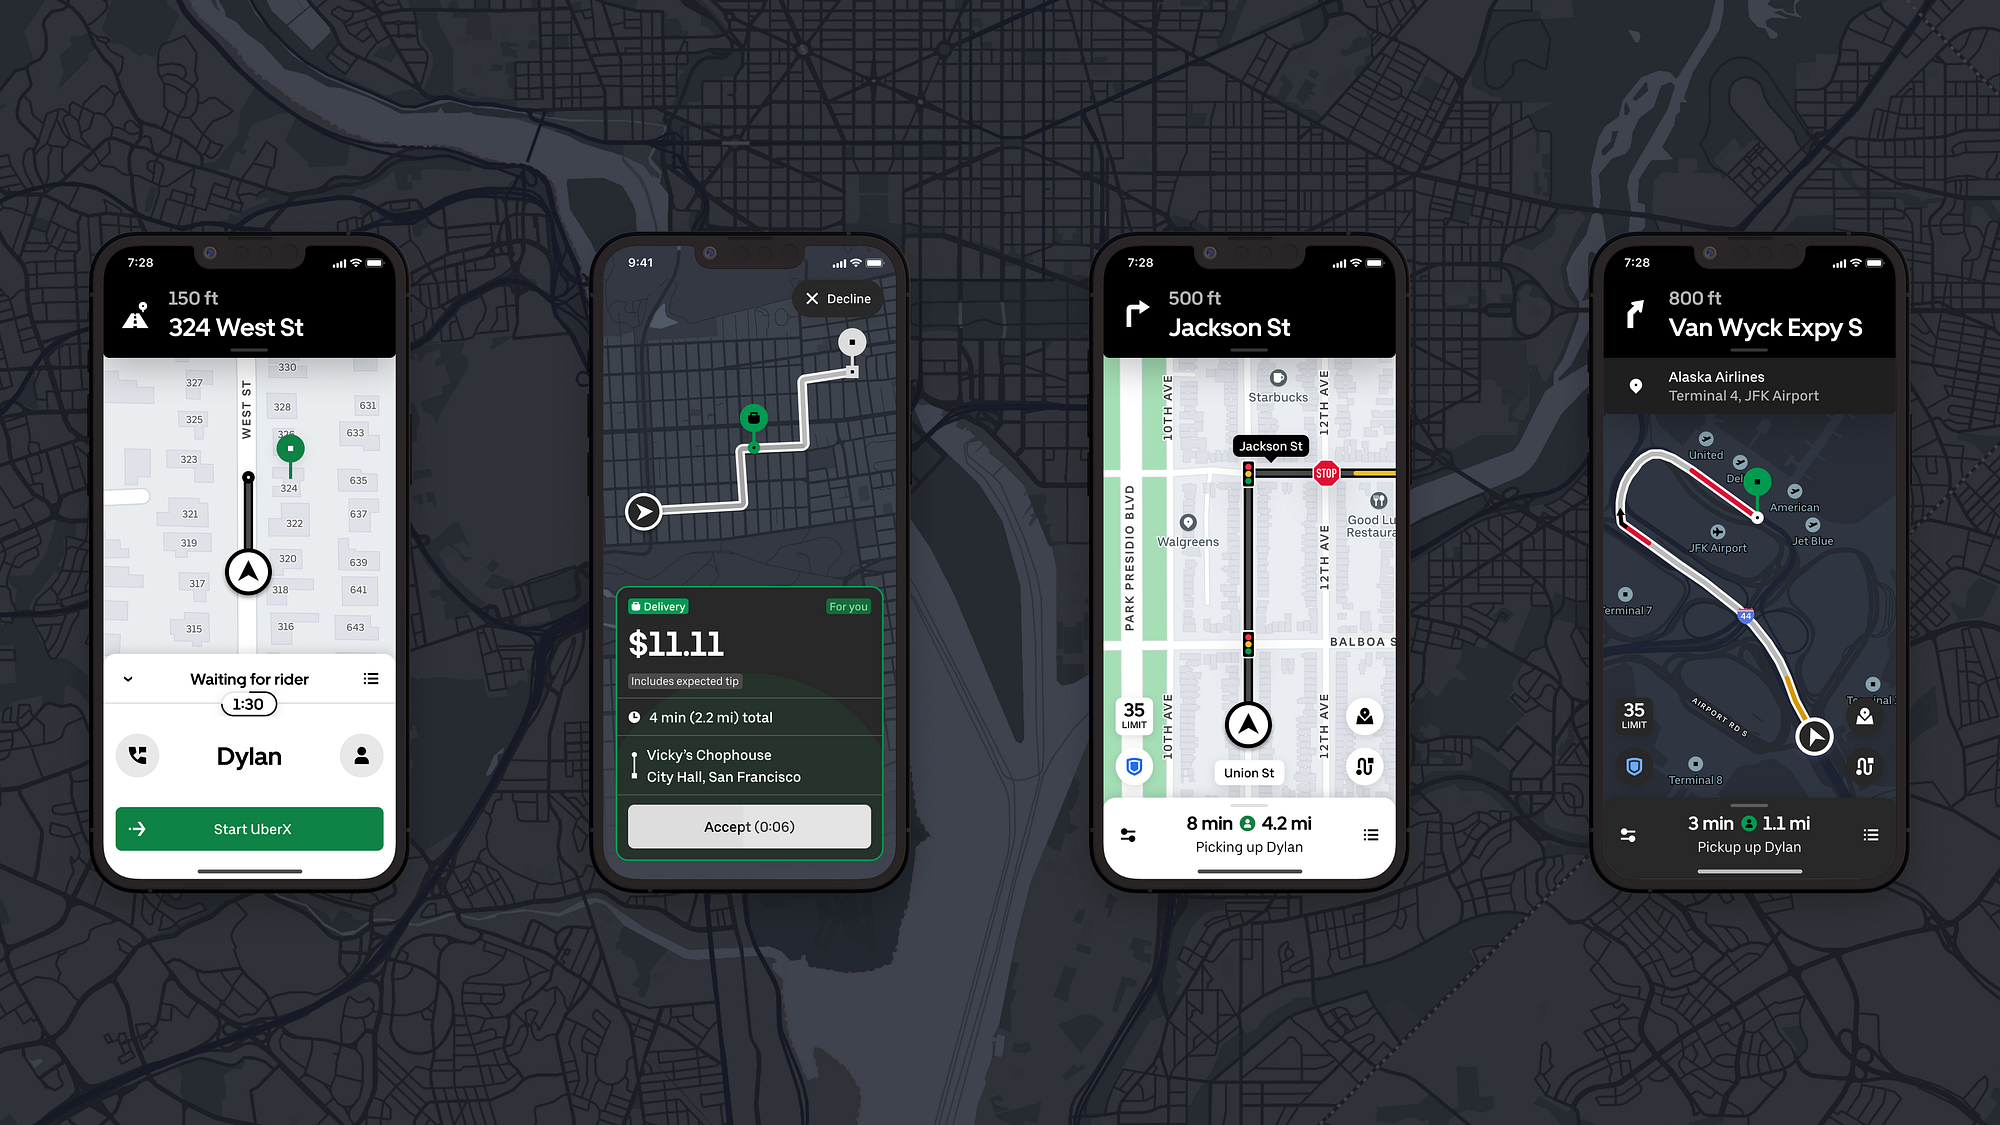
\includegraphics[width=0.8\textwidth]{imagenes/uber.png}
\caption{Seguimiento en tiempo real de un vehículo en Uber}
\label{fig:uber}
\end{figure}

Además, existen diversos Trabajos de Fin de Grado centrados en el desarrollo de aplicaciones móviles y el uso de tecnologías de geolocalización. Un ejemplo es el proyecto realizado por Mario Llorente Pérez \cite{marioTFG}, enfocado en una aplicación móvil relacionada con actividades deportivas y el uso de mapas y geolocalización. En trabajos como este puede observarse el importante papel que juega la localización en tiempo real y la necesidad de diseñar interfaces que permitan al usuario interactuar con la aplicación de forma sencilla.

Todas estas aplicaciones y trabajos constituyen ejemplos claros de que el seguimiento en tiempo real es una funcionalidad ampliamente utilizada, a pesar de que en el contexto de la Semana Santa sigue estando limitada y, cuando se ofrece, suele restringirse a entornos locales o presentar un nivel de precisión reducido.

Por tanto, su incorporación en una solución a nivel nacional conseguiría no solo mejorar la experiencia de los usuarios, sino también superar las limitaciones de las soluciones actuales en cuanto a la oferta de información precisa sobre el estado y la ubicación de las procesiones o eventos.
